\section*{ANALYSIS}\label{analysis}
\subsection*{FNPF}\label{fnpf}
The FNPF results have the benifit of having all the three states:
$\phi$, $\dot{\phi}$ and $\ddot{\phi}$. This means that these time
series can be inserted into the differential equation
(Eq.\ref{eq:roll_decay_equation_quadratic_a}) and the parameters
of the model can be estimated using Ordinary Least Square method (OLS),
solving the following regression:
\begin{equation}
y = X \cdot \beta + \epsilon
\label{eq:ols}
\end{equation}
where:
\begin{itemize}
\item $y$ is the dependent variable (also called *label*).
\item $\beta$ is a vector with the regressed parameters.
\item $X$ is a matrix containing the independent variables (also called *features*).
\end{itemize}
The roll decay equation can be expressed as a linear regression with
\begin{itemize}
\item $y$ : the roll angle acceleration $\ddot{\phi}$
\item $\beta$ : contains all the parameters : $B_1$, $B_2$, $C_1$...
\item $X$ : contains all the time varying features such as: $| \dot{\phi} | \dot{\phi} $ etc.
\end{itemize}
So the roll acceleration is put on the left hand side:
\begin{equation}
\begin{aligned}
- \ddot{\phi} = B_{1A} \dot{\phi} + B_{2A} \left|{\dot{\phi}}\right| \dot{\phi} + B_{3A} \dot{\phi}^{3} + C_{1A} \phi + C_{3A} \phi^{3} \\ + C_{5A} \phi^{5}
\end{aligned}
\label{eq:acceleration_equation_cubic}
\end{equation}
The equation for the acceleration
Eq.\ref{eq:acceleration_equation_cubic} can now be rewritten as
the linear regression in Eq.\ref{eq:ols}, where:
\begin{equation}
\beta = \left[\begin{matrix}B_{3A}\\C_{3A}\\C_{5A}\\B_{2A}\\B_{1A}\\C_{1A}\end{matrix}\right]
\label{eq:eq_beta}
\end{equation}
\begin{equation}
X = \left[\begin{matrix}\dot{\phi}^{3} & \phi^{3} & \phi^{5} & \left|{\dot{\phi}}\right| \dot{\phi} & \dot{\phi} & \phi\end{matrix}\right]
\label{eq:eq_X}
\end{equation}
\begin{equation}
y = - \ddot{\phi}
\label{eq:eq_y}
\end{equation}
The coefficients determined with Ordinary Least Square fit is shown in
Tab.\ref{tab:parameters}. The mean value of these coefficients
are presented togehter with 5\% confidence level intervalls.
\begin{table}[H]
\scriptsize
\center
\caption{Parameters estimation cubic model}
\label{tab:parameters1}
\begin{tabular}{|l|l|l|l|l|}
\hline\addlinespace
coeff & mean & $P_{value}$ & $conf_{lower}$ & $conf_{higher}$\\
B_3A & 0.098 & 0.0 & 0.072 & 0.124\\
\hlineC_3A & -5.522 & 0.0 & -5.807 & -5.236\\
C_5A & 254.093 & 0.0 & 244.923 & 263.264\\
B_2A & -0.062 & 0.0 & -0.076 & -0.047\\
B_1A & 0.016 & 0.0 & 0.014 & 0.018\\
C_1A & 6.116 & 0.0 & 6.114 & 6.118\\
\hline
\end{tabular}
\end{table}
\subsection*{Simulation}\label{simulation}
Fig.\ref{fig:sim_cubic} shows a simulation with the regressed
parameters together with the original data from the FNPF simulations.
\begin{figure}[H]
\begin{center}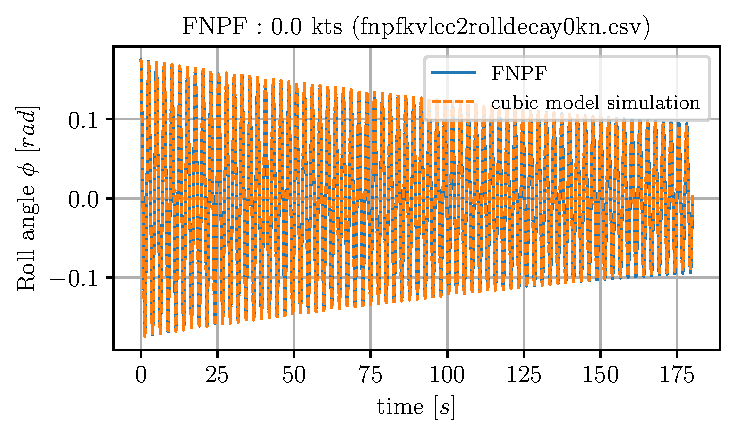
\includegraphics[width = 0.95\textwidth]{figures/sim_cubic.pdf}\end{center}
\vspace{-0.7cm}
\caption{Simulation of roll decay test with parameters from the cubic model.}
\label{fig:sim_cubic}
\end{figure}
\begin{equation}
- \ddot{\phi} = B_{1A} \dot{\phi} + C_{1A} \phi
\label{eq:Eq(-Derivative(phi(t), (t, 2)), B_1A*Derivative(phi(t), t) + C_1A*phi(t))}
\end{equation}
\begin{equation}
\beta = \left[\begin{matrix}B_{1A}\\C_{1A}\end{matrix}\right]
\label{eq:eq_beta2}
\end{equation}
\begin{equation}
X = \left[\begin{matrix}\dot{\phi} & \phi\end{matrix}\right]
\label{eq:eq_X2}
\end{equation}
\begin{table}[H]
\scriptsize
\center
\caption{Parameters estimation linear model}
\label{tab:parameters2}
\begin{tabular}{|l|l|l|l|l|}
\hline\addlinespace
coeff & mean & $P_{value}$ & $conf_{lower}$ & $conf_{higher}$\\
B_1A & 0.007 & 0.0 & 0.007 & 0.007\\
\hlineC_1A & 6.101 & 0.0 & 6.1 & 6.101\\
\hline
\end{tabular}
\end{table}
\begin{figure}[H]
\begin{center}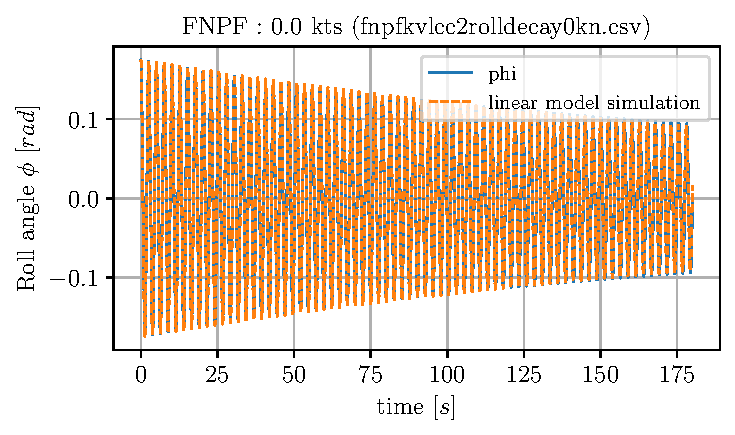
\includegraphics[width = 0.95\textwidth]{figures/sim_linear.pdf}\end{center}
\vspace{-0.7cm}
\caption{Simulation of roll decay test with parameters from the linear model.}
\label{fig:sim_linear}
\end{figure}
The coefficient of determination $R^2$ is very similar between the
cubic (0.997) and the linear model (0.989), when comparing simulated
roll signal with the corresponding data from FNPF.
\subsection*{Model tests}\label{model-tests}
Fig.\ref{fig:roll_decay_model_test} shows the roll signal from
one of the roll decay model tests. A sample from this signal as
indicated by the ``cut'' in Fig.\ref{fig:roll_decay_model_test}
is used to regress the roll damping. The roll velocity and acceleration
are however missing from this test data. This means that the regression
approach as used for the FNPF data cannot be used directly. Instead the
velocity and acceleration are first estimated using numerical gradient.
The acceleration and velocity signals estimated in this way are very
noisy as shown in Fig.\ref{fig:roll_velocity_and_acceleration},
where the roll angle measurement noise is included in the gradients.
Results from a regression with this noisy data is shown in
Fig.\ref{fig:roll_acceleration_ols}, where the numerical
acceleration and a 5\% confidence intervall is also shown.
Fig.\ref{fig:roll_acceleration_residual} shows the distribution
of the residual error.
\begin{figure}[H]
\begin{center}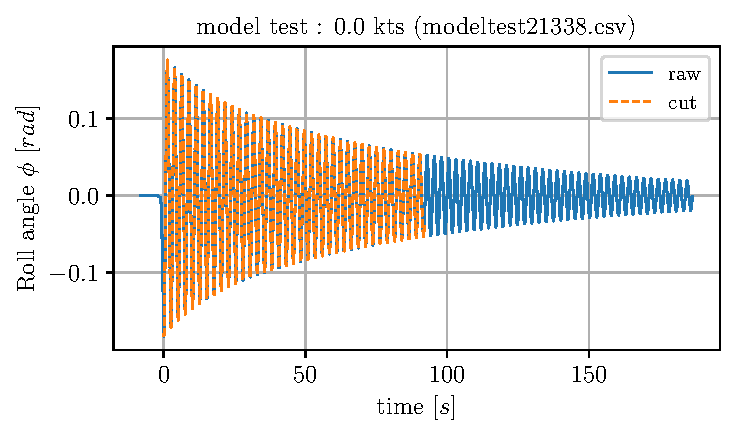
\includegraphics[width = 0.95\textwidth]{figures/roll_decay_model_test.pdf}\end{center}
\vspace{-0.7cm}
\caption{Roll decay model test}
\label{fig:roll_decay_model_test}
\end{figure}
\begin{table}[H]
\scriptsize
\center
\caption{Parameters estimation cubic model}
\label{tab:parameters3}
\begin{tabular}{|l|l|l|l|l|}
\hline\addlinespace
coeff & mean & $P_{value}$ & $conf_{lower}$ & $conf_{higher}$\\
B_3A & -0.262 & 0.958 & -10.069 & 9.544\\
\hlineC_3A & 14.386 & 0.786 & -89.472 & 118.245\\
C_5A & -382.877 & 0.829 & -3862.87 & 3097.115\\
B_2A & 0.222 & 0.932 & -4.891 & 5.335\\
B_1A & -0.006 & 0.985 & -0.622 & 0.61\\
C_1A & 6.035 & 0.0 & 5.412 & 6.657\\
\hline
\end{tabular}
\end{table}
\begin{table}[H]
\scriptsize
\center
\caption{Parameters estimation linear model}
\label{tab:parameters4}
\begin{tabular}{|l|l|l|l|l|}
\hline\addlinespace
coeff & mean & $P_{value}$ & $conf_{lower}$ & $conf_{higher}$\\
B_1A & 0.031 & 0.5 & -0.059 & 0.121\\
\hlineC_1A & 6.127 & 0.0 & 5.905 & 6.349\\
\hline
\end{tabular}
\end{table}
\begin{figure}[H]
\begin{center}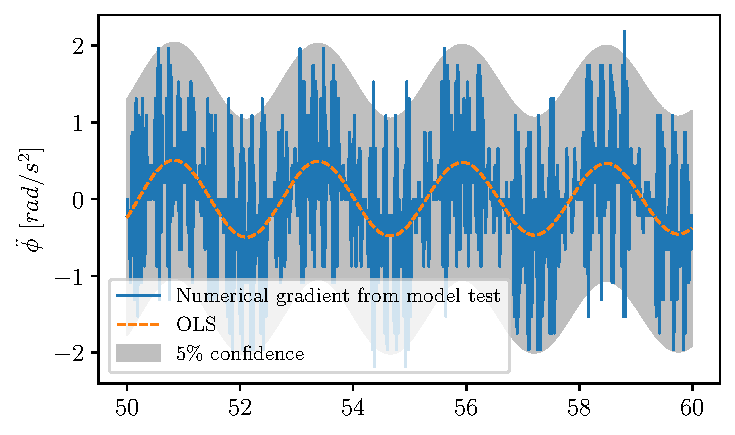
\includegraphics[width = 0.95\textwidth]{figures/roll_acceleration_ols.pdf}\end{center}
\vspace{-0.7cm}
\caption{Roll acceleration from numerical gradient and OLS regression}
\label{fig:roll_acceleration_ols}
\end{figure}
\begin{figure}[H]
\begin{center}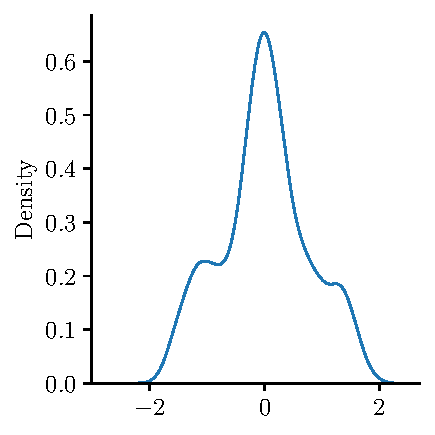
\includegraphics[width = 0.95\textwidth]{figures/roll_acceleration_residual.pdf}\end{center}
\vspace{-0.7cm}
\caption{Roll acceleration residual of linear model}
\label{fig:roll_acceleration_residual}
\end{figure}
The coefficient of determination $R^2$ is slightly higher for the
cubic model (0.971) compared to the the linear model (0.962), when
comparing simulated roll signal with the corresponding data from the
model test.
\subsection*{Validation}\label{validation}
The other model test at 0 knots (see
Fig.\ref{fig:other_roll_decay}) is used for validation of the
regression models.
\begin{figure}[H]
\begin{center}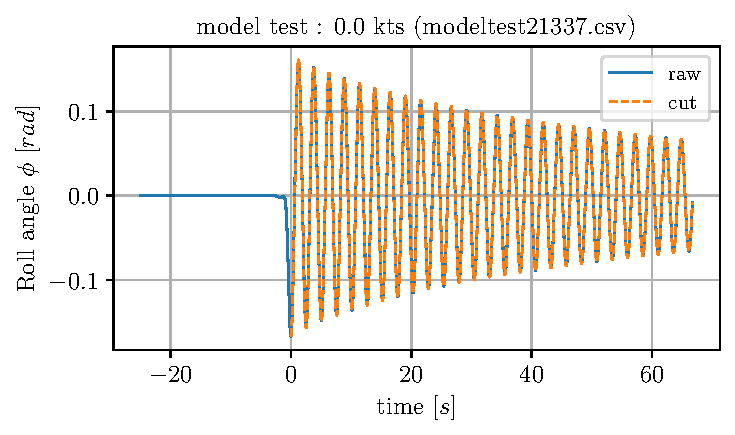
\includegraphics[width = 0.95\textwidth]{figures/other_roll_decay.pdf}\end{center}
\vspace{-0.7cm}
\caption{The other roll decay model test at 0 knots}
\label{fig:other_roll_decay}
\end{figure}
Fig.\ref{fig:other_roll_decay_sim} shows a comparison with this
model test and simulations with regressed parameters from the first
model test.
\begin{figure}[H]
\begin{center}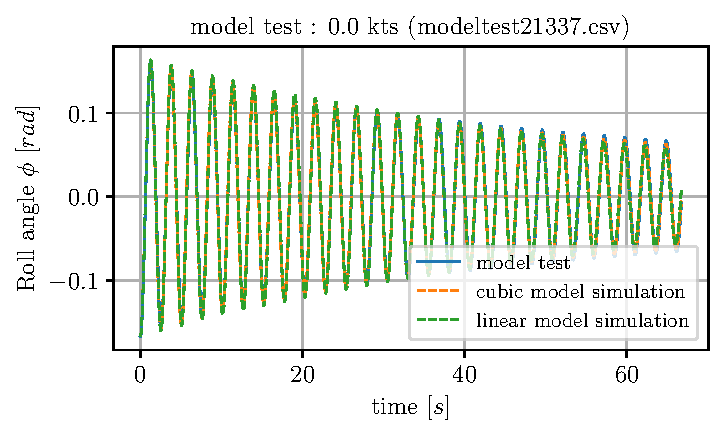
\includegraphics[width = 0.95\textwidth]{figures/other_roll_decay_sim.pdf}\end{center}
\vspace{-0.7cm}
\caption{The other roll decay model test compared with corresponding simulations with linear and cubic models regressed from the first model test.}
\label{fig:other_roll_decay_sim}
\end{figure}
The coefficient of determination $R^2$ is slightly lower for the cubic
model (0.98) compared to the the linear model (0.982), when comparing
simulated roll signal with the corresponding data from the model test.
